\documentclass[a4paper,12pt,openany]{scrreprt}
\usepackage[
	left=2.5cm, 
	right=4cm, 
    top=2.5cm, 
    bottom=2.8cm,
    footskip=10mm,
    headsep=5mm]{geometry}

\usepackage[
    colorlinks=true,
    citecolor=black,
    linkcolor=black,
    menucolor=black,
    urlcolor=black
]{hyperref}

\usepackage{scrhack}
\usepackage[utf8]{inputenc}
\usepackage[T1]{fontenc}
\usepackage{graphicx}
%\graphicspath{{images/}}
%\usepackage{fancyhdr}
\usepackage{lmodern}
\usepackage{color}
%\usepackage[table,dvipsnames]{xcolor}
\usepackage{transparent}
\usepackage[ngerman]{babel}
\usepackage{lipsum}
\usepackage[useregional]{datetime2}
\DTMlangsetup[de-DE]{monthyearsep={\space}}
\usepackage{setspace}
\onehalfspacing
\usepackage{tikz}
\usepackage{float}
\usepackage{amsmath}
\usepackage{amsfonts}
\usepackage{calc}
%\usepackage{subfig}
\usepackage{csquotes}
\MakeOuterQuote{"} 

%\usepackage[nottoc,notlot,notlof]{tocbibind}

\hypersetup{final}
\begin{document}

\pagestyle{empty}
\newgeometry{left=1.5cm,right=1.5cm,top=2cm,bottom=2cm}
\begin{center}

\Huge{\textbf{Universität Bielefeld}}

\LARGE{Fakultät für Linguistik und Literaturwissenschaft}

\vfill

\LARGE{\textbf{Hausarbeit}}

\Large

\href{https://ekvv.uni-bielefeld.de/sinfo/publ/modul/26797308}{23-LIN-BaLinS2}

\vfill

% On the Topic:

\vspace*{1cm}

\LARGE{\textbf{Unterschiede in der Phrasierung von gesprochenen und gesungenen Texten}\\\Large{am Beispiel zweier englischsprachiger Chor-Arrangements}}

\Large

\vfill

vorgelegt von

\vspace*{1cm}

\textbf{\href{https://fabianwohlgemuth.de}{Fabian Wohlgemuth}}

\vfill

$\begin{aligned}
\text{Begutachtet von:}&\ \text{Frau Prof. Dr. Petra Wagner}\\
% \text{Zweitgutachterin:}&\ \text{Frau Prof. Dr. Barbara Job}
\end{aligned}$

\vfill

\DTMlangsetup{showdayofmonth=false}
Bielefeld, \today
\DTMlangsetup{showdayofmonth=true}

\end{center}
\restoregeometry

\pagenumbering{Roman}

%\addcontentsline{toc}{section}{Danksagung}\setcounter{page}{2}\include{formalia/danksagung}
%\addcontentsline{toc}{section}{Abstract}\chapter*{Abstract}
\label{chap:Abstract}

% The following module paper looks at the current state of literature in the fields of language and music, to establish possible approaches to the interface between said fields.

%\addcontentsline{toc}{section}{Table of Contents}
\newpage
\tableofcontents

\newpage
\let\LaTeXStandardClearpage\clearpage
\let\clearpage\relax

%\begin{spacing}{1.1}
%\addcontentsline{toc}{section}{List of Figures/Tables}\listoffigures \listoftables
%\chapter*{Abkürzungsverzeichnis}
\label{chap:Abkürzungsverzeichnis}

\begin{acronym}[Bash]
% \acro{SMK}{Social Media Kommunikation}
\end{acronym}
%\end{spacing}

%\addtocontents{toc}{\vspace{\normalbaselineskip}}
%\addtocontents{toc}{\hrule}
%\addtocontents{toc}{\vspace{\normalbaselineskip}}
\let\clearpage\LaTeXStandardClearpage
\newpage
\pagenumbering{arabic}

\newpage
\chapter{Einleitung}
\label{chap:Einleitung}

% schriftliche Arbeit im Umfang von 10-15 Seiten

\begin{quote}
\textit{''Music is the universal language of mankind.''}
\\--- Henry Wadsworth Longfellow

\textit{''Wer hört auf die Worte, wo Töne siegen!''} 
\\--- Richard Strauss, Capriccio (Szene 3)
\end{quote}

\vspace{1cm}

Die vorliegende Hausarbeit wurde erstellt im Rahmen der Modulabschlussprüfung des Moduls 23-LIN-BaLinS2 im Bachelorstudium Linguistik mit Profil Sprache. Sie befasst sich mit Unterschieden zwischen gesungener und gesprochener Sprache und konzentriert sich in diesem Themenfeld auf die Phrasierung.

Durch Mitgliedschaften in diversen kleinen und großen Vokal-Ensembles, bin ich schon seit einiger Zeit in den Kreisen der Stimm-fokussierten Musik zu Hause. Aus eben selben Kreisen heraus ist die Motivation für diese Hausarbeit entstanden, die Sprache und Musik zu verbinden versucht.

In \autoref{sec:Phrasierung} werde ich definieren, was unter Phrasierung zu verstehen ist.
Im Anschluss werde ich in \autoref{chap:Datensatz} den \nameref{chap:Datensatz} beschreiben. Dieser besteht aus zwei englischsprachigen Chor-Arrangements. Ich werde die Struktur der Stücke umreißen und sowohl die Liedtexte als auch die relevanten Melodien herausarbeiten.
Nach Erläuterung des Datensatzes werde ich in \autoref{chap:Methodik} erläutern, mit welcher Methodik ich die Texte und Melodien analysieren werde. Hier greife ich auf theoretische Modelle und praktische Anwendungen der Computerlinguistik zurück.
Die \nameref{chap:Ergebnisse} werde ich in \autoref{chap:Ergebnisse} aufzeigen und ausarbeiten.
Anschließend werden die Ergebnisse in \autoref{chap:Diskussion} diskutiert. Hier zeige ich, welche Erkenntnisse aus meinen Untersuchungen gewonnen werden konnten und welchen Wert sie innerhalb der Forschung einnehmen können.
In \autoref{chap:Fazit und Ausblick} werde ich ein Fazit aus der Arbeit ziehen und einen Ausblick geben, inwieweit die Forschungen ausgeweitet werden können. Außerdem werde ich darauf eingehen, welche Probleme während der Arbeit aufkamen und wie ich die Arbeit hätte verbessern können.

% Welches Ziel verfolge ich?

% Was ist das Problem?

% Eingrenzung und Abgrenzung des Themas

% Aufbau erklärt

% Roter Faden einlieiten

% Forschungsinteresse begründen?




\section{Phrasierung}
\label{sec:Phrasierung}

Bei der Phrasierung handelt es sich um die Strukturierung längerer sprachlicher Äußerungen in kleinere Einheiten. Getrennt sind diese Einheiten von sogenannten prosodischen Phrasengrenzen. In der geschriebenen Sprache sind Interpunktions-Zeichen gute Anhaltspunkte für Phrasengrenzen. Wird ein Text vorgelesen stimmen Satzzeichen meist mit diesen Phrasengrenzen überein. So werden am Satzende und gelegentlich auch bei Kommata und Konjunktionen Sprechpausen gemacht \cite{trouvain2018}. Trouvain beschreibt außerdem den Zusammenhang von Sprechpausen und syntaktischen Phrasengrenzen. Eine längere sprachliche Äußerung ohne die benannten Satzzeichen, die zur Phrasierung führen, äußert sich diese durch eine Pause, nahe der Äußerungs-Mitte \cite{gee1983performance}.

Im musikalischen Kontext passiert eine Phrasierung durch Pausenzeichen, wie zum Beispiel $\AcPa$, $\ViPa$ oder $\HaPa$. Bei den Zeichen handelt es sich um Achtelpausen, Viertelpausen und halbe Pausen, die entsprechend des Tempos und der Taktart des Stückes jeweils einen achte, viertel beziehungsweise halben Schlag einnehmen.
\chapter{Datensatz}
\label{chap:Datensatz}
\pagestyle{plain}

Untersuchungsgrundlage der Hausarbeit sind die zwei im Folgenden vorgestellten Chor-Arrangements. Die Noten der beiden Stücke befinden sich in ihrer Gesamtheit im \nameref{chap:Anhang}. An dieser Stelle werden nur Text und für die Ausarbeitung relevante Ausschnitte der Noten präsentiert.

\section{Run To You}

Bei dem ersten Stück handelt es sich um \textit{Run To You}, geschrieben von der A Cappella Gruppe \textit{Pentatonix} in Zusammenarbeit mit Ben Bram. \textit{Run To You} ist ein fünfstimmiges Chor-Arrangement für Sopran, Alt, Tenor, Bariton und Bass. Das Stück ist aufgeteilt in zwei Strophen (Studierziffern A und C), gefolgt von jeweils einem Refrain (Studierziffern B und D). Der zweite Refrain mündet in die Bridge (Studierziffer E). Das Stück endet mit einem leicht veränderten Refrain (Studierziffer F), dessen Ende gesummt wird.

\subsection*{Text}

\begin{verbatim}
[Strophe 1]
A light in the room
It was you who was standing there
Tried, it was true
As your glance met my stare
But your heart drifted off
Like the land split by sea
I tried to go, to follow
To kneel down at your feet

[Refrain]
I'll run, I'll run, I'll run, run to you
I'll run, I'll run, I'll run, run to you

[Strophe 2]
I've been settling scores
I've been fighting so long
But I've lost your war
And our kingdom is gone
How shall I win back your heart
Which was mine?
I have broken bones
And tattered clothes
I've run out of time

[Refrain]

[Bridge]
Oh, I will break down the gates of heaven
A thousand angels stand waiting for me
Oh take my heart and I'll lay down my weapons
Break my shackles to set me free

[Refrain]
\end{verbatim}

\subsection*{Melodie}

In diesem Stück alterniert die Melodie-Stimme zwischen Tenor und Alt. Die Strophen (Studierziffern A und C) werden von der Tenor-Stimme, Refrain und Bridge (Studierziffern B, D, E, F) von der Alt-Stimme geführt.

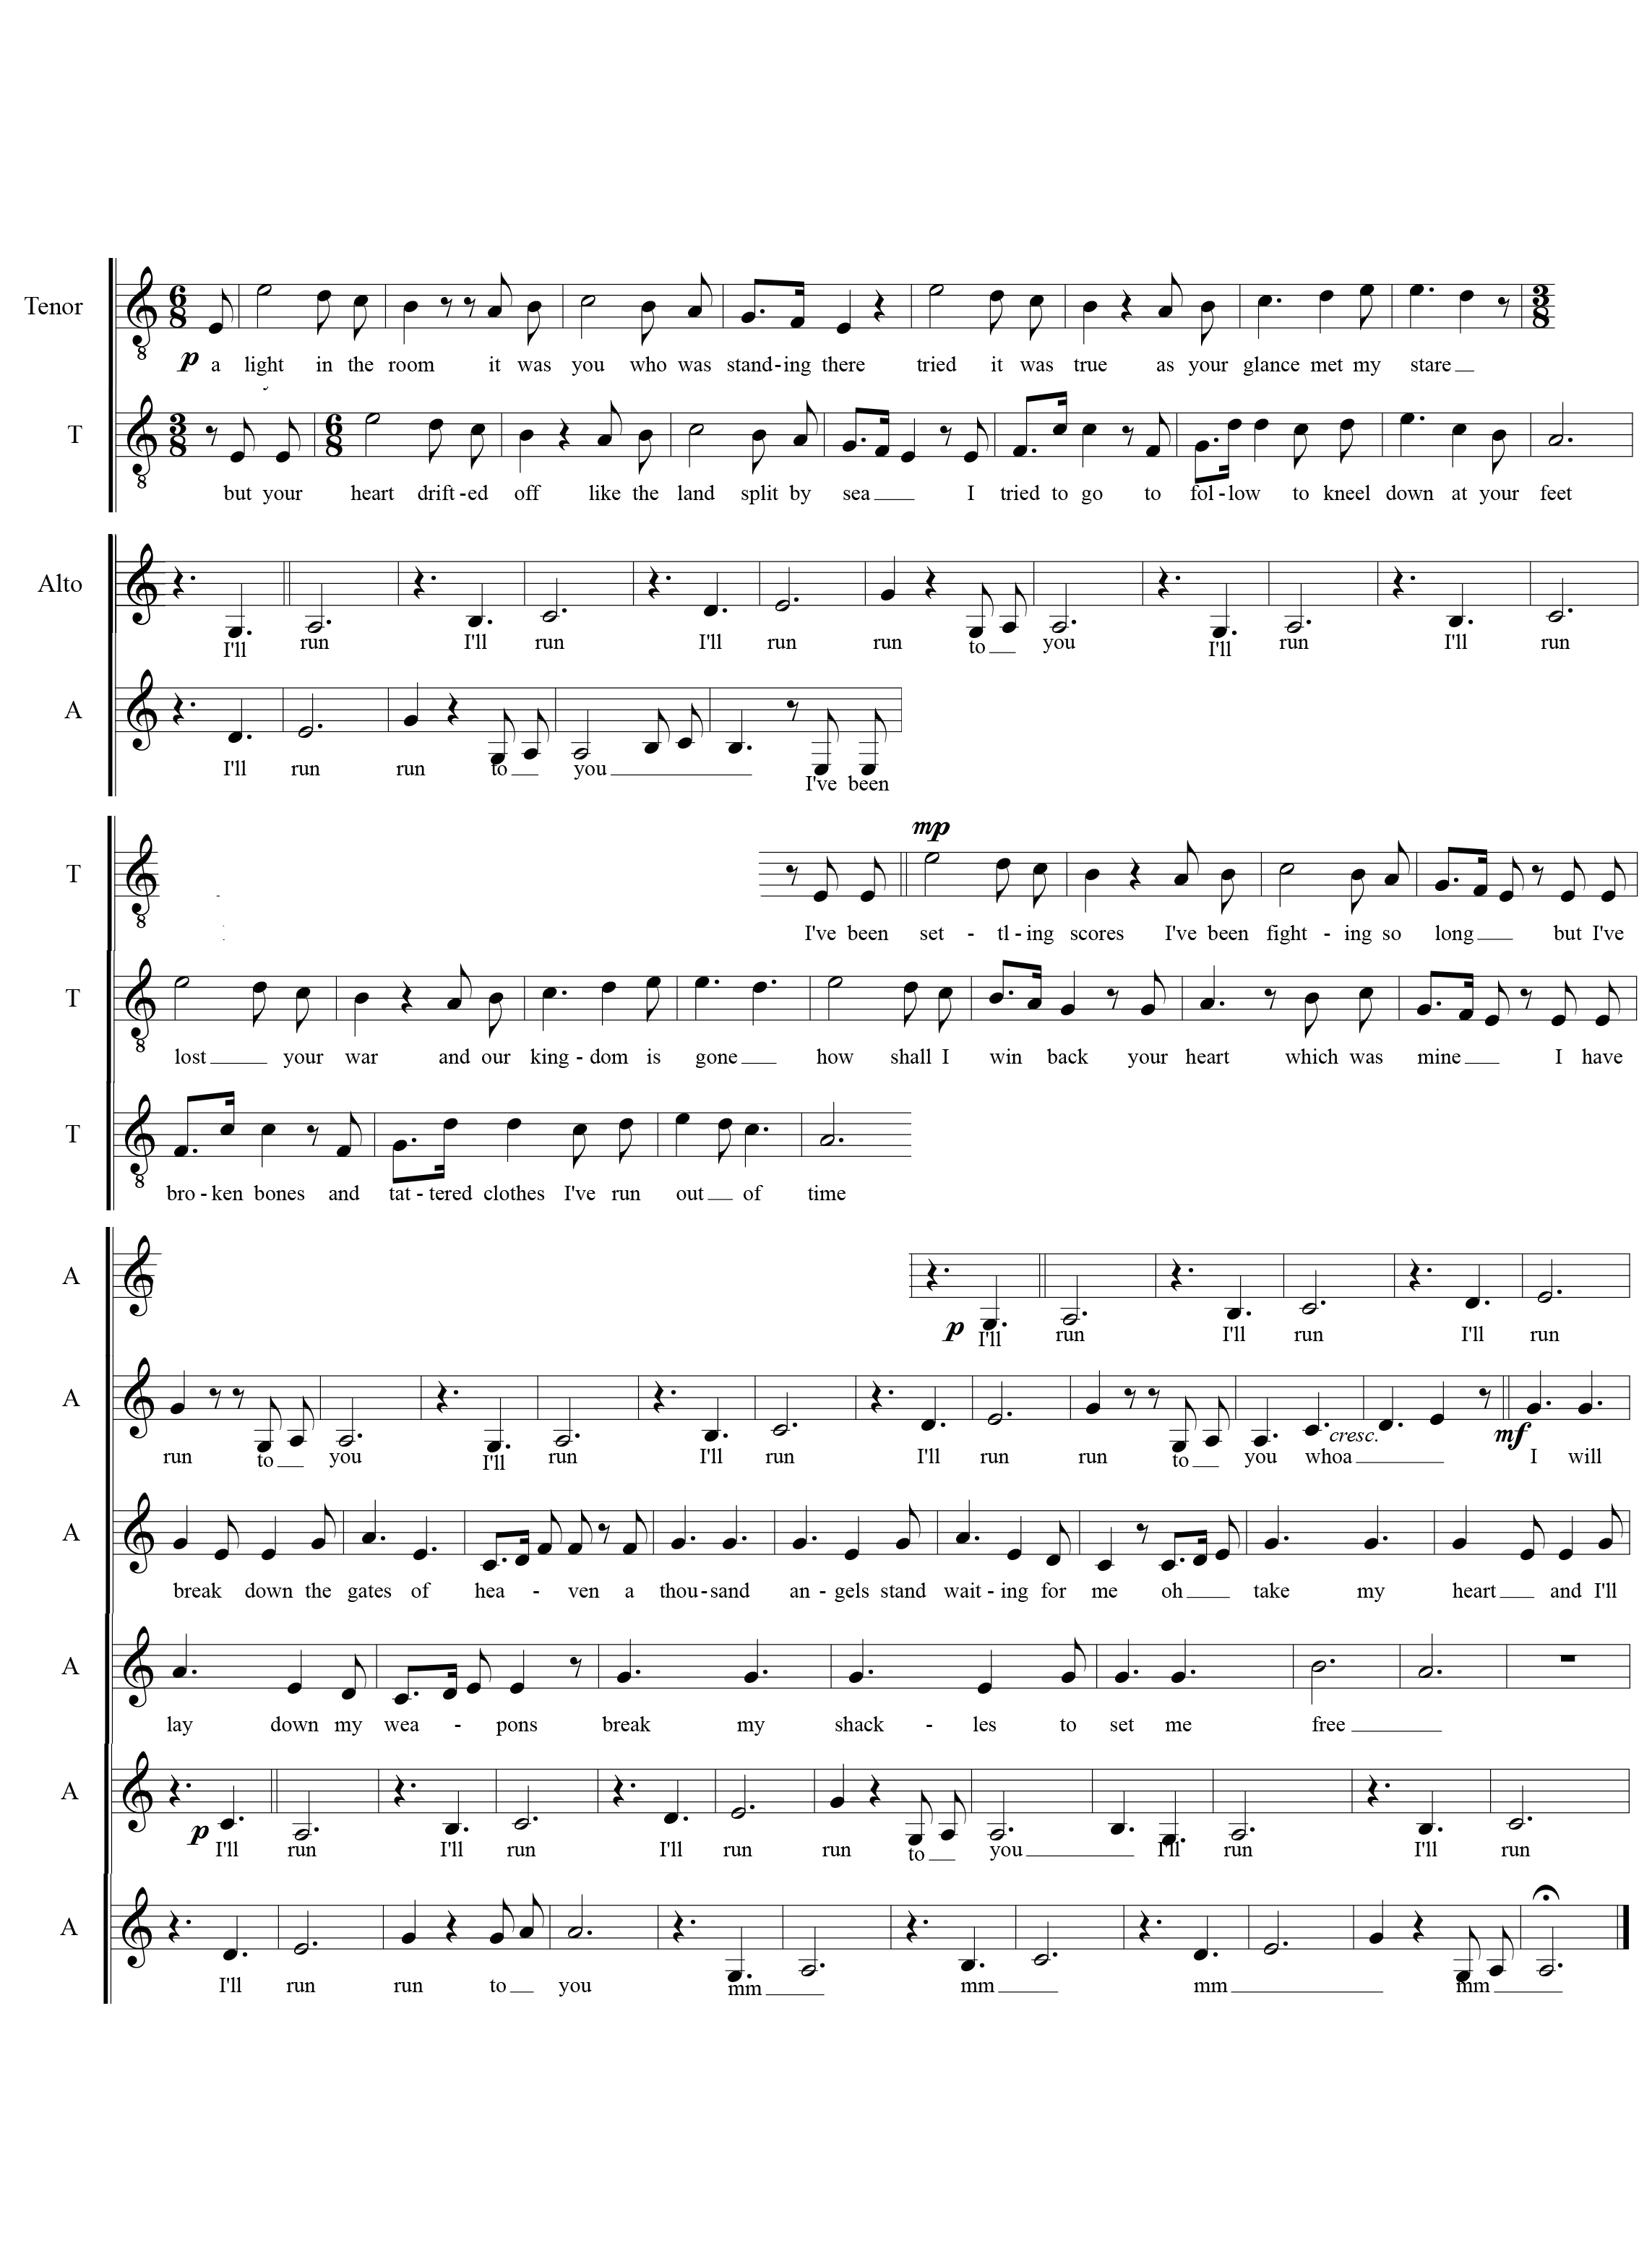
\includegraphics[width=\textwidth]{resources/arrangements/Run To You - Melody.png}
\label{appendix:Run To You}
 

\section{Fields Of Gold}

Das zweite Stück ist \textit{Fields Of Gold}, geschrieben von Gordon Sumner — bekannt unter dem Künstlernamen \textit{Sting} — und arrangiert von Greg Jasperse. Bei dem vorliegenden Arrangement handelt es sich um einen Satz für Sopran, Alt, Tenor und Bass. Das Stück besteht aus sechs Strophen, wobei sich zwischen der vierten und fünften Strophe eine Bridge befindet.

\begin{verbatim}
[Strophe 1]
You'll remember me when the west wind moves
Upon the fields of barley
You'll forget the sun in his jealous sky
As we walk in fields of gold

[Strophe 2]
So she took her love for to gaze awhile
Upon the fields of barley
In his arms she fell as her hair came down
Among the fields of gold

[Strophe 3]
Will you stay with me? Will you be my love?
Upon the fields of barley
We'll forget the sun in his jealous sky
As we lie in fields of gold

[Strophe 4]
See the west wind move like a lover so
Upon the fields of barley
Feel her body rise when you kiss her mouth
Among the fields of gold

[Bridge]
I never made promises lightly
And there have been some that I've broken
But I swear in the days still left
We'll walk in fields of gold
We'll walk in fields of gold

[Strophe 5]
Many years have passed since those summer days
Upon the fields of barley
See the children run as the sun goes down
Among the fields of gold

[Strophe 6]
You'll remember me when the west wind moves
Upon the fields of barley
You can tell the sun in his jealous sky
When we walked in fields of gold
When we walked in fields of gold
When we walked in fields of gold
\end{verbatim}
\chapter{Methodik}
\label{chap:Methodik}
\pagestyle{plain}

Im folgenden Abschnitt werde ich die zwei Stücke auf Ihre Phrasierung untersuchen. Dabei starte ich mit der Melodie von \textit{Run To You}, die sich aus den Noten mithilfe von Pausenzeichen in gesungene Phrasen einteilen lässt. Dazu nutze ich die klassische Baumstruktur, die auch \cite{lerdahl1983generative} nutzen und adaptiere diese für die gesungene Phrasierung auf die simpelste Form. Dabei nummeriere ich die Phrasen, um sie später in Kombination mit der Strophen-Nummer eindeutig identifizieren zu können. 

Für eine bessere Übersichtlichkeit, verbinde ich die Phrasen der Melodie nicht miteinander. Auch \cite{hayes1996role} nutzen die Baum-Notation und bedienen sich außerdem der Raster-Notation aus \cite{liberman1975intonational} für die Notation des Rhythmus. Da ich mich in dieser Arbeit nur auf die Untersuchung der Phrasierung beschränke, sind diese Mehr-Informationen jedoch von geringerer Relevanz.

\tiny 

\section*{Run To You}

\subsection*{Melodie}

HOW? MIT DEN PAUSEN

\subsubsection*{Strophe 1}

\Tree [.Phrase-1 \qroof{A light in the room}. ] 
\Tree [.Phrase-2 \qroof{It was you who was standing there}. ] 
\Tree [.Phrase-3 \qroof{Tried, it was true}. ] 
\Tree [.Phrase-4 \qroof{As your glance met my stare}. ] 
\Tree [.Phrase-5 \qroof{But your heart drifted off}. ] 
\Tree [.Phrase-6 \qroof{Like the land split by sea}. ] 
\Tree [.Phrase-7 \qroof{I tried to go,}. ] 
\Tree [.Phrase-8 \qroof{to follow. To kneel down at your feet}. ] 

\subsubsection*{Refrain 1}

\Tree [.Phrase-1 \qroof{I'll run}. ] 
\Tree [.Phrase-2 \qroof{I'll run}. ] 
\Tree [.Phrase-3 \qroof{I'll run}. ] 
\Tree [.Phrase-4 \qroof{run to you}. ] 
\Tree [.Phrase-5 \qroof{I'll run}. ] 
\Tree [.Phrase-6 \qroof{I'll run}. ] 
\Tree [.Phrase-7 \qroof{I'll run}. ] 
\Tree [.Phrase-8 \qroof{run to you}. ] 

\subsubsection*{Strophe 2}

\Tree [.Phrase-1 \qroof{I've been settling scores}. ] 
\Tree [.Phrase-2 \qroof{I've been fighting so long}. ] 
\Tree [.Phrase-3 \qroof{But I've lost your war}. ] 
\Tree [.Phrase-4 \qroof{And our kingdom is gone. How shall I win back}. ] 
\Tree [.Phrase-5 \qroof{Your heart}. ] 
\Tree [.Phrase-6 \qroof{which was mine}. ] 
\Tree [.Phrase-7 \qroof{I have broken bones}. ] 
\Tree [.Phrase-8 \qroof{and tattered clothes. I've run out of time}. ] 

\subsubsection*{Refrain 2 (siehe oben)}

\subsubsection*{Bridge}

\Tree [.Phrase-1 \qroof{I will break down the gates of heaven}. ] 
\Tree [.Phrase-3 \qroof{A thousand angels stand waiting for me}. ] 
\Tree [.Phrase-4 \qroof{Ooh take my heart (take my heart) And I'll lay down my weapons}. ] 
\Tree [.Phrase-5 \qroof{Break my shackles to set me free}. ] 

\subsubsection*{Refrain 3 (siehe oben)}




\subsection*{Text}

HOW?

\subsubsection*{Strophe 1}

\Tree [.Phrase-1 \qroof{A light in the room}. ] 
\Tree [.Phrase-2 \qroof{It was you who was standing there}. ] 
\Tree [.Phrase-3 \qroof{Tried, it was true}. ] 
\Tree [.Phrase-4 \qroof{As your glance met my stare}. ] 
\Tree [.Phrase-5 \qroof{But your heart drifted off}. ] 
\Tree [.Phrase-6 \qroof{Like the land split by sea}. ] 
\Tree [.Phrase-7 \qroof{I tried to go,}. ] 
\Tree [.Phrase-8 \qroof{to follow}. ] 
\Tree [.Phrase-9 \qroof{To kneel down at your feet}. ] 

\subsubsection*{Refrain 1}

\Tree [.Phrase-1 \qroof{I'll run}. ] 
\Tree [.Phrase-2 \qroof{I'll run}. ] 
\Tree [.Phrase-3 \qroof{I'll run}. ] 
\Tree [.Phrase-4 \qroof{run to you}. ] 
\Tree [.Phrase-5 \qroof{I'll run}. ] 
\Tree [.Phrase-6 \qroof{I'll run}. ] 
\Tree [.Phrase-7 \qroof{I'll run}. ] 
\Tree [.Phrase-8 \qroof{run to you}. ] 

\subsubsection*{Strophe 2}

\Tree [.Phrase-1 \qroof{I've been settling scores}. ] 
\Tree [.Phrase-2 \qroof{I've been fighting so long}. ] 
\Tree [.Phrase-3 \qroof{But I've lost your war}. ] 
\Tree [.Phrase-4 \qroof{And our kingdom is gone.}. ] 
\Tree [.Phrase-5 \qroof{How shall I win back your heart which was mine}. ] 
\Tree [.Phrase-6 \qroof{I have broken bones and tattered clothes}. ] 
\Tree [.Phrase-7 \qroof{I've run out of time}. ] 

\subsubsection*{Refrain 2 (siehe oben)}

\subsubsection*{Bridge}

\Tree [.Phrase-1 \qroof{I will break down the gates of heaven}. ] 
\Tree [.Phrase-2 \qroof{A thousand angels stand waiting for me}. ] 
\Tree [.Phrase-3 \qroof{Take my heart and I'll lay down my weapons}. ] 
\Tree [.Phrase-4 \qroof{Break my shackles to set me free}. ] 

\subsubsection*{Refrain 3 (siehe oben)}















\normalsize
\chapter{Ergebnisse}
\label{chap:Ergebnisse}
\pagestyle{plain}


\chapter{Diskussion}
\label{chap:Diskussion}
\pagestyle{plain}


\chapter{Fazit und Ausblick}
\label{chap:Fazit und Ausblick}

% Ergebnisse zusammenfassen und bewerten - Beantworten der Fragen aus der Einleitung - Ausblick / Offene Fragen / Angrenzende Themengebiete
% KEINE neuen Erkenntnisse / Thesen



%% ---------------------------------------%%

%\pagestyle{plain}

\addtocontents{toc}{\vspace{\normalbaselineskip}}
\addtocontents{toc}{\hrule}
\addtocontents{toc}{\vspace{\normalbaselineskip}}

\renewcommand{\bibname}{Literaturverzeichnis}
\pagenumbering{Roman}
\bibliographystyle{apalike}
\begin{doublespace}
\bibliography{mp_balins2.bib}
\end{doublespace}

\let\clearpage\LaTeXStandardClearpage
\addcontentsline{toc}{chapter}{Literaturverzeichnis}
\clearpage
\addcontentsline{toc}{chapter}{Eigenständigkeitserklärung}
\begin{doublespace}
\newgeometry{left=2.5cm,right=2.5cm,top=2cm,bottom=2cm}
%\doublespacing

{\let\clearpage\relax \chapter*{\centerline{Declaration of Authorship}}}
\label{chap:Declaration of Authorship}

\vspace*{1cm}

\setlength{\parindent}{0pt}
I hereby declare authorship of the module paper on hand. The module paper is entirely my own original work except where otherwise indicated. I am aware of the University's regulations concerning plagiarism, including those regulations concerning disciplinary actions that may result from plagiarism. Any use of the works of any other author, in any form, is properly acknowledged at their point of use.
\vspace*{2cm}

Bielefeld, \today \hfill \hrulefill

\hspace*{0mm}\phantom{Bielefeld, } 
\hfill Fabian Wohlgemuth\hspace*{1cm}
\restoregeometry
\end{doublespace}

%\addcontentsline{toc}{chapter}{Appendix}
%\chapter*{Anhang}
\label{chap:Anhang}

\begin{itemize}
  \item Run To You
  \item Fields Of Gold
\end{itemize}

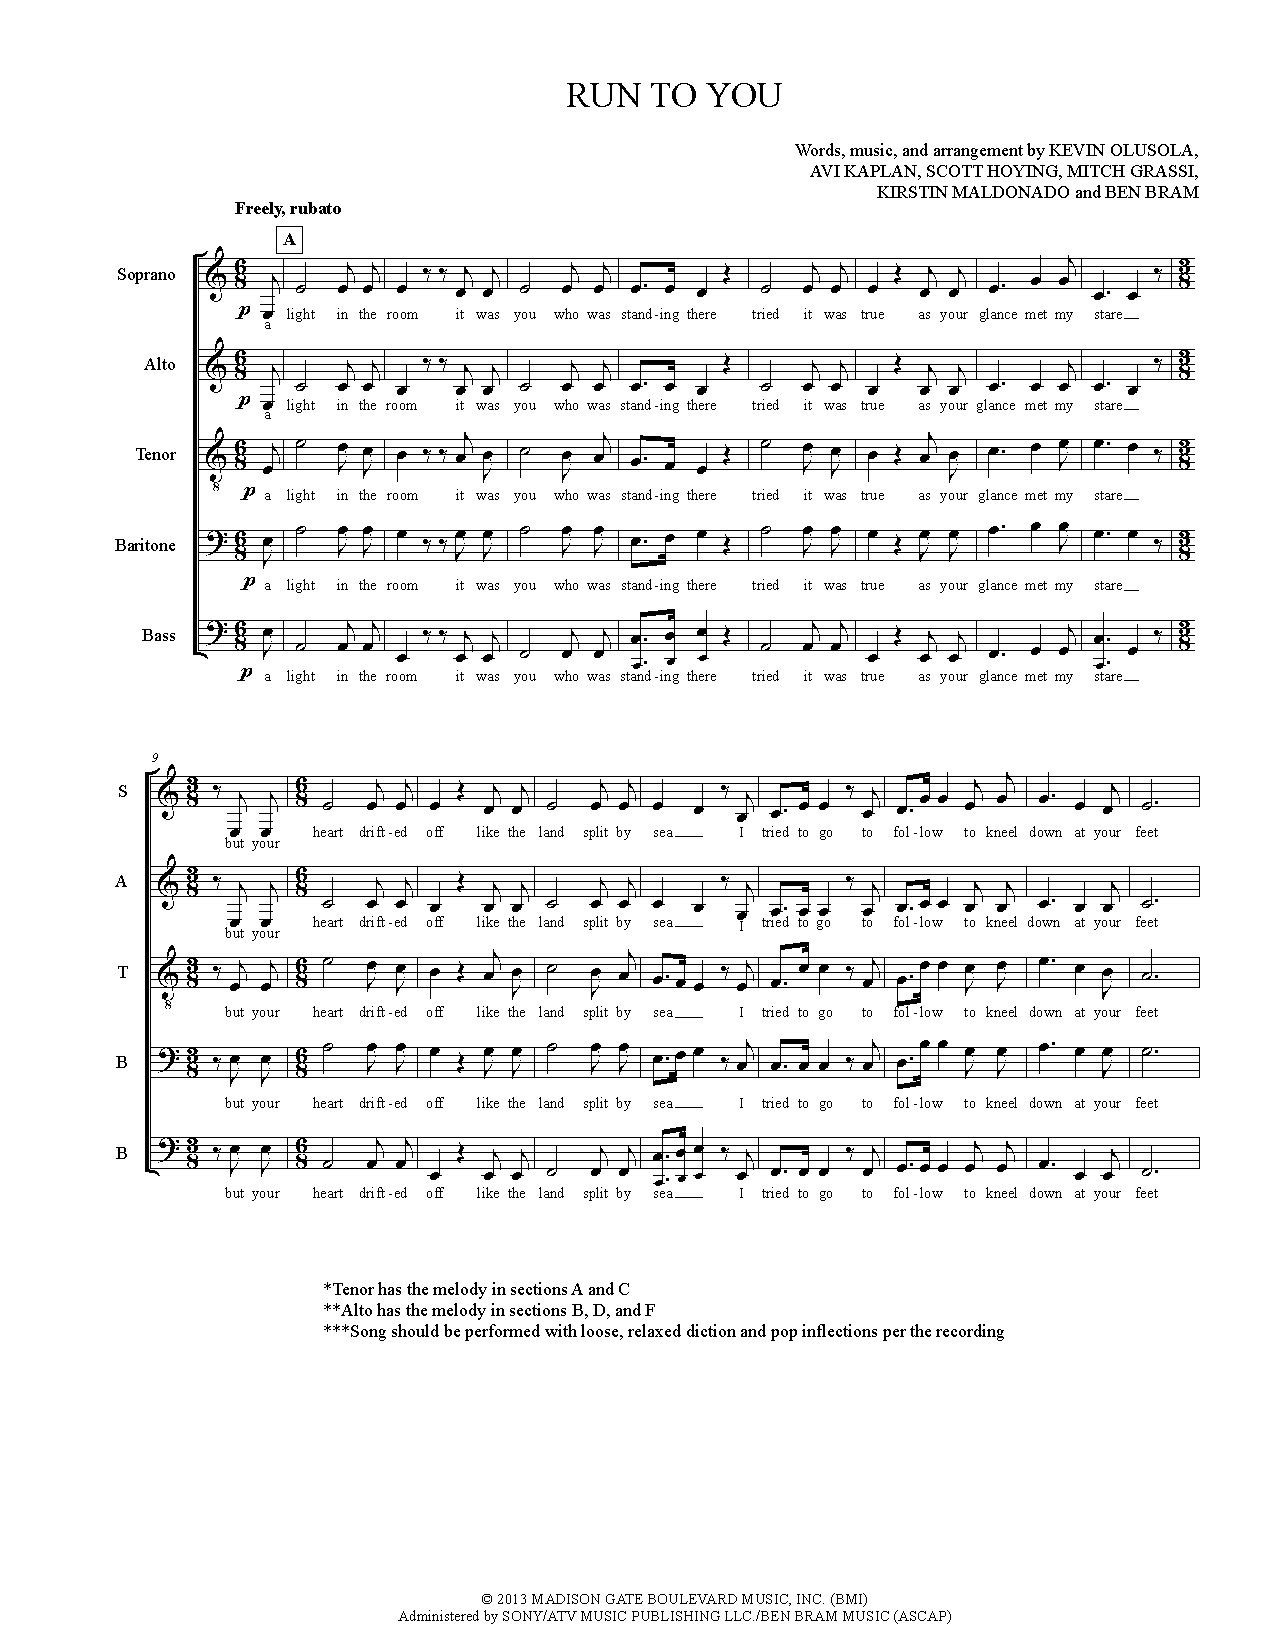
\includepdf[pages=-]{resources/arrangements/Run To You.pdf}
\label{appendix:Run To You}

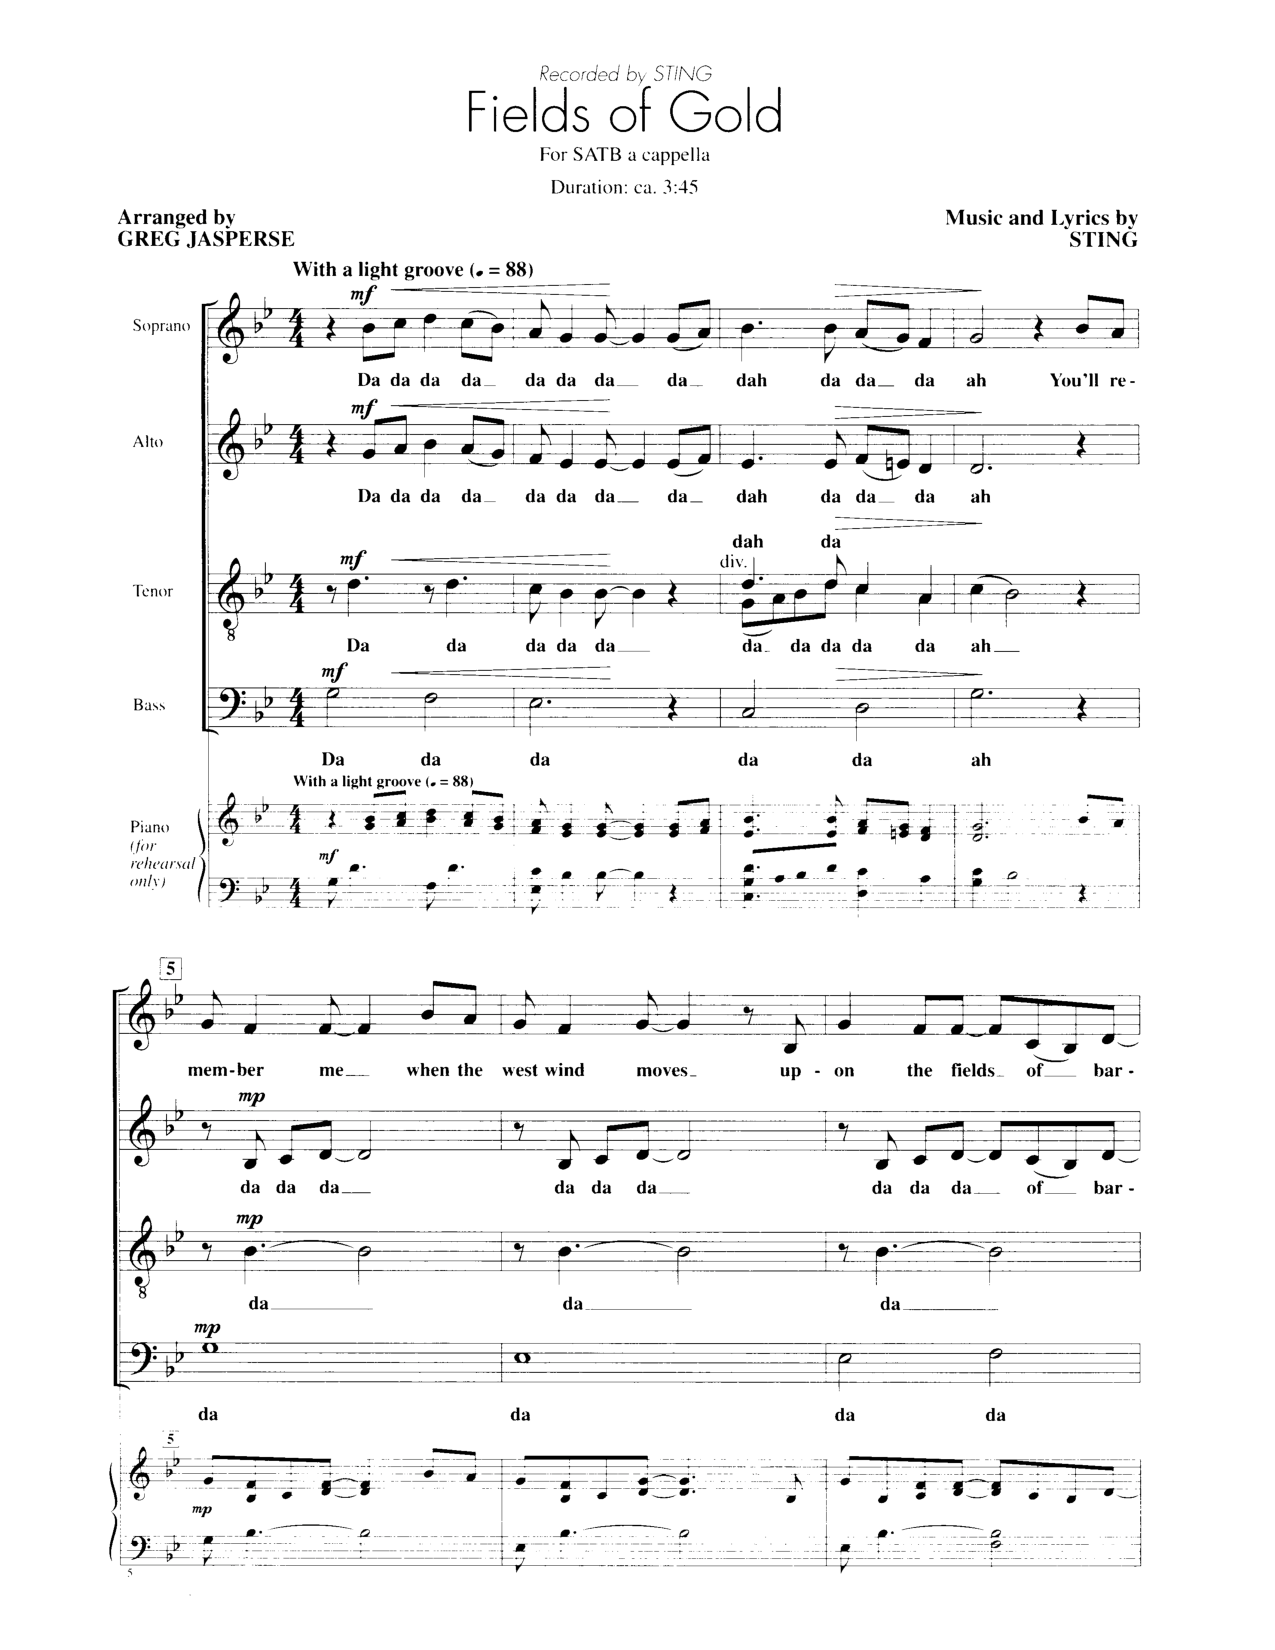
\includepdf[pages=-]{resources/arrangements/Fields Of Gold.pdf}
\label{appendix:Fields Of Gold} 


\end{document}
